\documentclass[1p]{elsarticle_modified}
%\bibliographystyle{elsarticle-num}

%\usepackage[colorlinks]{hyperref}
%\usepackage{abbrmath_seonhwa} %\Abb, \Ascr, \Acal ,\Abf, \Afrak
\usepackage{amsfonts}
\usepackage{amssymb}
\usepackage{amsmath}
\usepackage{amsthm}
\usepackage{scalefnt}
\usepackage{amsbsy}
\usepackage{kotex}
\usepackage{caption}
\usepackage{subfig}
\usepackage{color}
\usepackage{graphicx}
\usepackage{xcolor} %% white, black, red, green, blue, cyan, magenta, yellow
\usepackage{float}
\usepackage{setspace}
\usepackage{hyperref}

\usepackage{tikz}
\usetikzlibrary{arrows}

\usepackage{multirow}
\usepackage{array} % fixed length table
\usepackage{hhline}

%%%%%%%%%%%%%%%%%%%%%
\makeatletter
\renewcommand*\env@matrix[1][\arraystretch]{%
	\edef\arraystretch{#1}%
	\hskip -\arraycolsep
	\let\@ifnextchar\new@ifnextchar
	\array{*\c@MaxMatrixCols c}}
\makeatother %https://tex.stackexchange.com/questions/14071/how-can-i-increase-the-line-spacing-in-a-matrix
%%%%%%%%%%%%%%%

\usepackage[normalem]{ulem}

\newcommand{\msout}[1]{\ifmmode\text{\sout{\ensuremath{#1}}}\else\sout{#1}\fi}
%SOURCE: \msout is \stkout macro in https://tex.stackexchange.com/questions/20609/strikeout-in-math-mode

\newcommand{\cancel}[1]{
	\ifmmode
	{\color{red}\msout{#1}}
	\else
	{\color{red}\sout{#1}}
	\fi
}

\newcommand{\add}[1]{
	{\color{blue}\uwave{#1}}
}

\newcommand{\replace}[2]{
	\ifmmode
	{\color{red}\msout{#1}}{\color{blue}\uwave{#2}}
	\else
	{\color{red}\sout{#1}}{\color{blue}\uwave{#2}}
	\fi
}

\newcommand{\Sol}{\mathcal{S}} %segment
\newcommand{\D}{D} %diagram
\newcommand{\A}{\mathcal{A}} %arc


%%%%%%%%%%%%%%%%%%%%%%%%%%%%%5 test

\def\sl{\operatorname{\textup{SL}}(2,\Cbb)}
\def\psl{\operatorname{\textup{PSL}}(2,\Cbb)}
\def\quan{\mkern 1mu \triangleright \mkern 1mu}

\theoremstyle{definition}
\newtheorem{thm}{Theorem}[section]
\newtheorem{prop}[thm]{Proposition}
\newtheorem{lem}[thm]{Lemma}
\newtheorem{ques}[thm]{Question}
\newtheorem{cor}[thm]{Corollary}
\newtheorem{defn}[thm]{Definition}
\newtheorem{exam}[thm]{Example}
\newtheorem{rmk}[thm]{Remark}
\newtheorem{alg}[thm]{Algorithm}

\newcommand{\I}{\sqrt{-1}}
\begin{document}

%\begin{frontmatter}
%
%\title{Boundary parabolic representations of knots up to 8 crossings}
%
%%% Group authors per affiliation:
%\author{Yunhi Cho} 
%\address{Department of Mathematics, University of Seoul, Seoul, Korea}
%\ead{yhcho@uos.ac.kr}
%
%
%\author{Seonhwa Kim} %\fnref{s_kim}}
%\address{Center for Geometry and Physics, Institute for Basic Science, Pohang, 37673, Korea}
%\ead{ryeona17@ibs.re.kr}
%
%\author{Hyuk Kim}
%\address{Department of Mathematical Sciences, Seoul National University, Seoul 08826, Korea}
%\ead{hyukkim@snu.ac.kr}
%
%\author{Seokbeom Yoon}
%\address{Department of Mathematical Sciences, Seoul National University, Seoul, 08826,  Korea}
%\ead{sbyoon15@snu.ac.kr}
%
%\begin{abstract}
%We find all boundary parabolic representation of knots up to 8 crossings.
%
%\end{abstract}
%\begin{keyword}
%    \MSC[2010] 57M25 
%\end{keyword}
%
%\end{frontmatter}

%\linenumbers
%\tableofcontents
%
\newcommand\colored[1]{\textcolor{white}{\rule[-0.35ex]{0.8em}{1.4ex}}\kern-0.8em\color{red} #1}%
%\newcommand\colored[1]{\textcolor{white}{ #1}\kern-2.17ex	\textcolor{white}{ #1}\kern-1.81ex	\textcolor{white}{ #1}\kern-2.15ex\color{red}#1	}

{\Large $\underline{12a_{0759}~(K12a_{0759})}$}

\setlength{\tabcolsep}{10pt}
\renewcommand{\arraystretch}{1.6}
\vspace{1cm}\begin{tabular}{m{100pt}>{\centering\arraybackslash}m{274pt}}
\multirow{5}{120pt}{
	\centering
	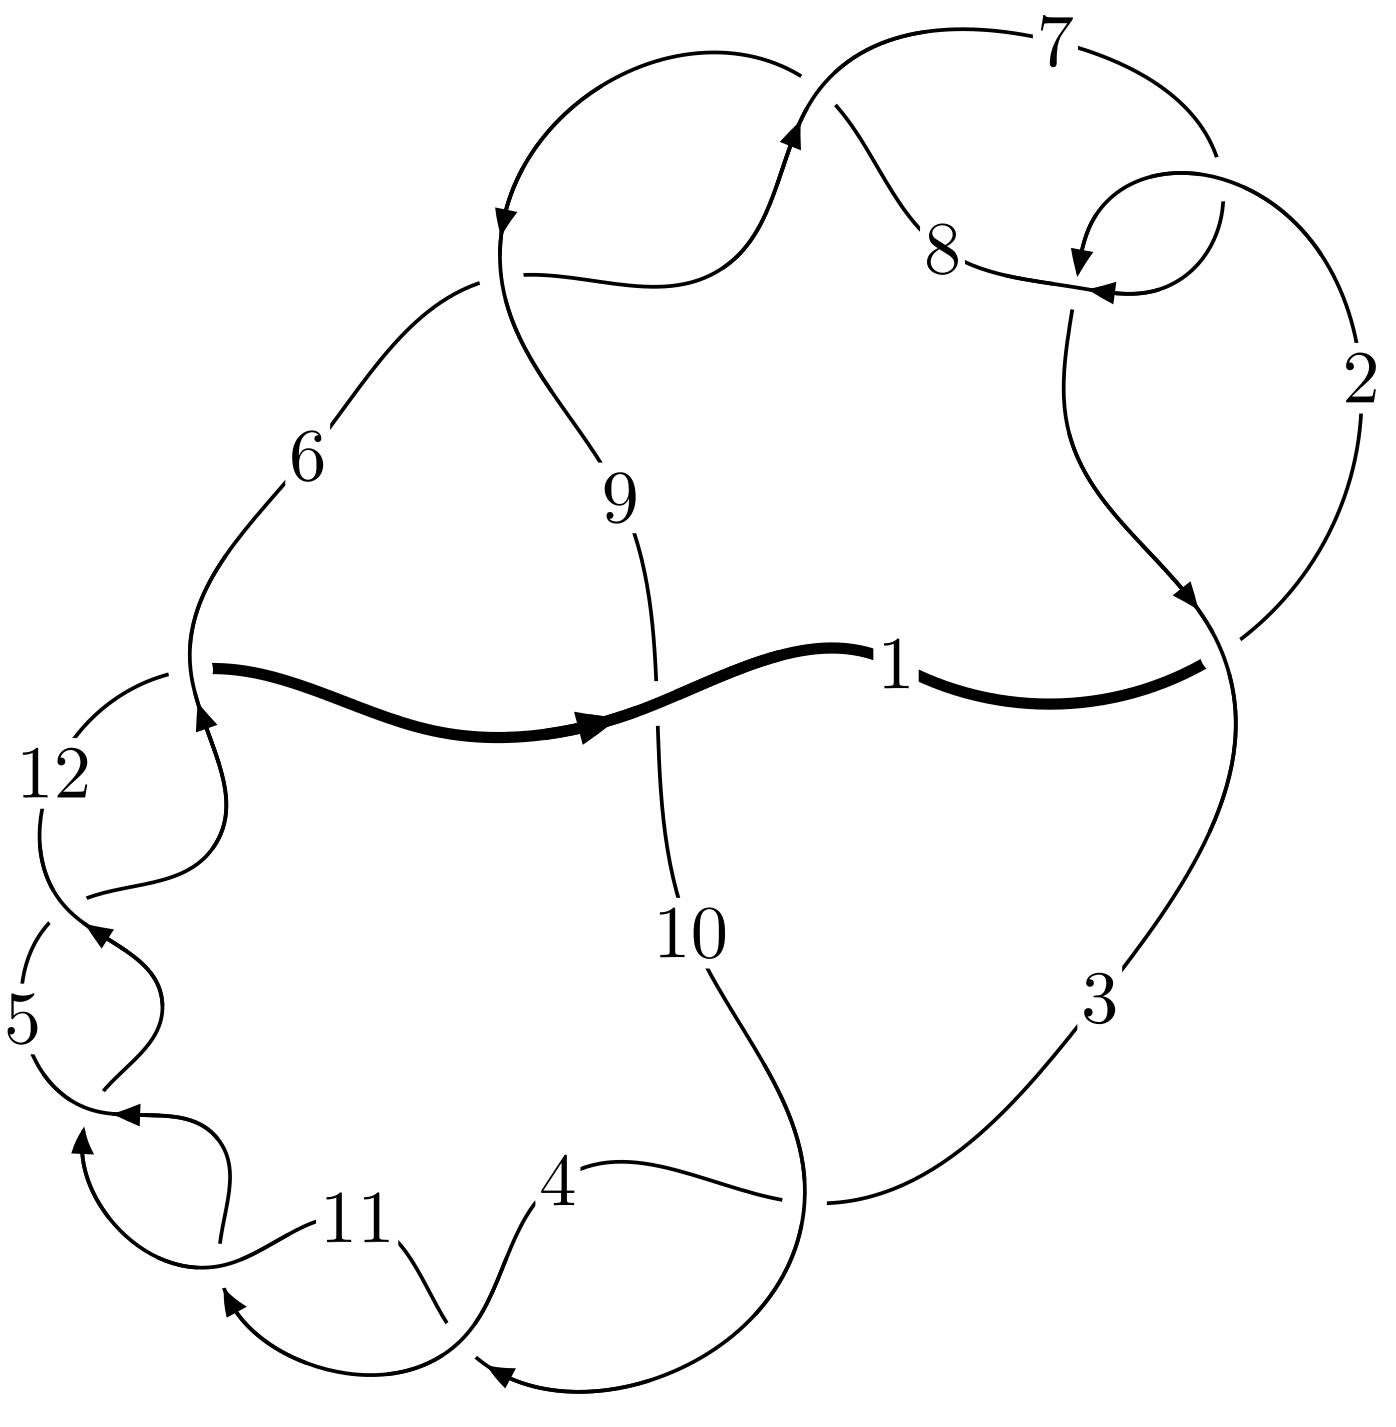
\includegraphics[width=112pt]{../../../GIT/diagram.site/Diagrams/png/1560_12a_0759.png}\\
\ \ \ A knot diagram\footnotemark}&
\allowdisplaybreaks
\textbf{Linearized knot diagam} \\
\cline{2-2}
 &
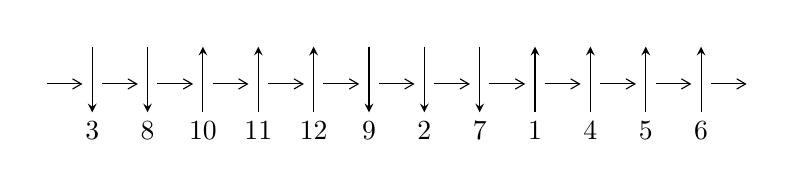
\begin{tikzpicture}[x=20pt, y=17pt]
	% nodes
	\node (C0) at (0, 0) {};
	\node (C1) at (1, 0) {};
	\node (C1U) at (1, +1) {};
	\node (C1D) at (1, -1) {3};

	\node (C2) at (2, 0) {};
	\node (C2U) at (2, +1) {};
	\node (C2D) at (2, -1) {8};

	\node (C3) at (3, 0) {};
	\node (C3U) at (3, +1) {};
	\node (C3D) at (3, -1) {10};

	\node (C4) at (4, 0) {};
	\node (C4U) at (4, +1) {};
	\node (C4D) at (4, -1) {11};

	\node (C5) at (5, 0) {};
	\node (C5U) at (5, +1) {};
	\node (C5D) at (5, -1) {12};

	\node (C6) at (6, 0) {};
	\node (C6U) at (6, +1) {};
	\node (C6D) at (6, -1) {9};

	\node (C7) at (7, 0) {};
	\node (C7U) at (7, +1) {};
	\node (C7D) at (7, -1) {2};

	\node (C8) at (8, 0) {};
	\node (C8U) at (8, +1) {};
	\node (C8D) at (8, -1) {7};

	\node (C9) at (9, 0) {};
	\node (C9U) at (9, +1) {};
	\node (C9D) at (9, -1) {1};

	\node (C10) at (10, 0) {};
	\node (C10U) at (10, +1) {};
	\node (C10D) at (10, -1) {4};

	\node (C11) at (11, 0) {};
	\node (C11U) at (11, +1) {};
	\node (C11D) at (11, -1) {5};

	\node (C12) at (12, 0) {};
	\node (C12U) at (12, +1) {};
	\node (C12D) at (12, -1) {6};
	\node (C13) at (13, 0) {};

	% arrows
	\draw[->,>={angle 60}]
	(C0) edge (C1) (C1) edge (C2) (C2) edge (C3) (C3) edge (C4) (C4) edge (C5) (C5) edge (C6) (C6) edge (C7) (C7) edge (C8) (C8) edge (C9) (C9) edge (C10) (C10) edge (C11) (C11) edge (C12) (C12) edge (C13) ;	\draw[->,>=stealth]
	(C1U) edge (C1D) (C2U) edge (C2D) (C3D) edge (C3U) (C4D) edge (C4U) (C5D) edge (C5U) (C6U) edge (C6D) (C7U) edge (C7D) (C8U) edge (C8D) (C9D) edge (C9U) (C10D) edge (C10U) (C11D) edge (C11U) (C12D) edge (C12U) ;
	\end{tikzpicture} \\
\hhline{~~} \\& 
\textbf{Solving Sequence} \\ \cline{2-2} 
 &
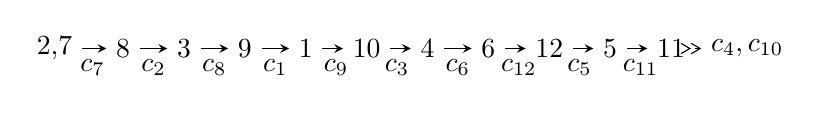
\begin{tikzpicture}[x=22pt, y=7pt]
	% node
	\node (A0) at (-1/8, 0) {2,7};
	\node (A1) at (1, 0) {8};
	\node (A2) at (2, 0) {3};
	\node (A3) at (3, 0) {9};
	\node (A4) at (4, 0) {1};
	\node (A5) at (5, 0) {10};
	\node (A6) at (6, 0) {4};
	\node (A7) at (7, 0) {6};
	\node (A8) at (8, 0) {12};
	\node (A9) at (9, 0) {5};
	\node (A10) at (10, 0) {11};
	\node (C1) at (1/2, -1) {$c_{7}$};
	\node (C2) at (3/2, -1) {$c_{2}$};
	\node (C3) at (5/2, -1) {$c_{8}$};
	\node (C4) at (7/2, -1) {$c_{1}$};
	\node (C5) at (9/2, -1) {$c_{9}$};
	\node (C6) at (11/2, -1) {$c_{3}$};
	\node (C7) at (13/2, -1) {$c_{6}$};
	\node (C8) at (15/2, -1) {$c_{12}$};
	\node (C9) at (17/2, -1) {$c_{5}$};
	\node (C10) at (19/2, -1) {$c_{11}$};
	\node (A11) at (45/4, 0) {$c_{4},c_{10}$};

	% edge
	\draw[->,>=stealth]	
	(A0) edge (A1) (A1) edge (A2) (A2) edge (A3) (A3) edge (A4) (A4) edge (A5) (A5) edge (A6) (A6) edge (A7) (A7) edge (A8) (A8) edge (A9) (A9) edge (A10) ;
	\draw[->>,>={angle 60}]	
	(A10) edge (A11);
\end{tikzpicture} \\ 

\end{tabular} \\

\footnotetext{
The image of knot diagram is generated by the software ``\textbf{Draw programme}" developed by Andrew Bartholomew(\url{http://www.layer8.co.uk/maths/draw/index.htm\#Running-draw}), where we modified some parts for our purpose(\url{https://github.com/CATsTAILs/LinksPainter}).
}\phantom \\ \newline 
\centering \textbf{Ideals for irreducible components\footnotemark of $X_{\text{par}}$} 
 
\begin{align*}
I^u_{1}&=\langle 
u^{30}- u^{29}+\cdots- u-1\rangle \\
\\
\end{align*}
\raggedright * 1 irreducible components of $\dim_{\mathbb{C}}=0$, with total 30 representations.\\
\footnotetext{All coefficients of polynomials are rational numbers. But the coefficients are sometimes approximated in decimal forms when there is not enough margin.}
\newpage
\renewcommand{\arraystretch}{1}
\centering \section*{I. $I^u_{1}= \langle u^{30}- u^{29}+\cdots- u-1 \rangle$}
\flushleft \textbf{(i) Arc colorings}\\
\begin{tabular}{m{7pt} m{180pt} m{7pt} m{180pt} }
\flushright $a_{2}=$&$\begin{pmatrix}0\\u\end{pmatrix}$ \\
\flushright $a_{7}=$&$\begin{pmatrix}1\\0\end{pmatrix}$ \\
\flushright $a_{8}=$&$\begin{pmatrix}1\\u^2\end{pmatrix}$ \\
\flushright $a_{3}=$&$\begin{pmatrix}- u\\- u^3+u\end{pmatrix}$ \\
\flushright $a_{9}=$&$\begin{pmatrix}- u^2+1\\u^2\end{pmatrix}$ \\
\flushright $a_{1}=$&$\begin{pmatrix}u^3\\u^5- u^3+u\end{pmatrix}$ \\
\flushright $a_{10}=$&$\begin{pmatrix}u^{10}- u^8+2 u^6- u^4- u^2+1\\u^{12}-2 u^{10}+4 u^8-4 u^6+3 u^4\end{pmatrix}$ \\
\flushright $a_{4}=$&$\begin{pmatrix}u^{19}-2 u^{17}+6 u^{15}-8 u^{13}+9 u^{11}-6 u^9+4 u^5-3 u^3\\u^{21}-3 u^{19}+9 u^{17}-16 u^{15}+24 u^{13}-25 u^{11}+21 u^9-10 u^7+3 u^5- u^3+u\end{pmatrix}$ \\
\flushright $a_{6}=$&$\begin{pmatrix}u^4- u^2+1\\- u^4\end{pmatrix}$ \\
\flushright $a_{12}=$&$\begin{pmatrix}- u^{13}+2 u^{11}-5 u^9+6 u^7-6 u^5+4 u^3- u\\u^{13}- u^{11}+3 u^9-2 u^7+2 u^5- u^3+u\end{pmatrix}$ \\
\flushright $a_{5}=$&$\begin{pmatrix}- u^{22}+3 u^{20}+\cdots-2 u^2+1\\u^{22}-2 u^{20}+\cdots-4 u^4+u^2\end{pmatrix}$ \\
\flushright $a_{11}=$&$\begin{pmatrix}- u^{28}+3 u^{26}+\cdots- u^2+1\\- u^{29}+u^{28}+\cdots- u-1\end{pmatrix}$\\&\end{tabular}
\flushleft \textbf{(ii) Obstruction class $= -1$}\\~\\
\flushleft \textbf{(iii) Cusp Shapes $= -4 u^{29}+16 u^{27}-4 u^{26}-60 u^{25}+12 u^{24}+148 u^{23}-44 u^{22}-304 u^{21}+88 u^{20}+508 u^{19}-160 u^{18}-692 u^{17}+212 u^{16}+796 u^{15}-224 u^{14}-736 u^{13}+168 u^{12}+568 u^{11}-80 u^{10}-344 u^9+180 u^7+24 u^6-84 u^5+32 u^3-8 u^2-12 u+6$}\\~\\
\newpage\renewcommand{\arraystretch}{1}
\flushleft \textbf{(iv) u-Polynomials at the component}\newline \\
\begin{tabular}{m{50pt}|m{274pt}}
Crossings & \hspace{64pt}u-Polynomials at each crossing \\
\hline $$\begin{aligned}c_{1},c_{6},c_{8}\end{aligned}$$&$\begin{aligned}
&u^{30}+7 u^{29}+\cdots+5 u+1
\end{aligned}$\\
\hline $$\begin{aligned}c_{2},c_{7}\end{aligned}$$&$\begin{aligned}
&u^{30}+u^{29}+\cdots+u-1
\end{aligned}$\\
\hline $$\begin{aligned}c_{3},c_{4},c_{5}\\c_{10},c_{11},c_{12}\end{aligned}$$&$\begin{aligned}
&u^{30}+u^{29}+\cdots- u-1
\end{aligned}$\\
\hline $$\begin{aligned}c_{9}\end{aligned}$$&$\begin{aligned}
&u^{30}-7 u^{29}+\cdots+521 u-295
\end{aligned}$\\
\hline
\end{tabular}\\~\\
\newpage\renewcommand{\arraystretch}{1}
\flushleft \textbf{(v) Riley Polynomials at the component}\newline \\
\begin{tabular}{m{50pt}|m{274pt}}
Crossings & \hspace{64pt}Riley Polynomials at each crossing \\
\hline $$\begin{aligned}c_{1},c_{6},c_{8}\end{aligned}$$&$\begin{aligned}
&y^{30}+33 y^{29}+\cdots+39 y+1
\end{aligned}$\\
\hline $$\begin{aligned}c_{2},c_{7}\end{aligned}$$&$\begin{aligned}
&y^{30}-7 y^{29}+\cdots-5 y+1
\end{aligned}$\\
\hline $$\begin{aligned}c_{3},c_{4},c_{5}\\c_{10},c_{11},c_{12}\end{aligned}$$&$\begin{aligned}
&y^{30}-43 y^{29}+\cdots-5 y+1
\end{aligned}$\\
\hline $$\begin{aligned}c_{9}\end{aligned}$$&$\begin{aligned}
&y^{30}-23 y^{29}+\cdots-1109241 y+87025
\end{aligned}$\\
\hline
\end{tabular}\\~\\
\newpage\flushleft \textbf{(vi) Complex Volumes and Cusp Shapes}
$$\begin{array}{c|c|c}  
\text{Solutions to }I^u_{1}& \I (\text{vol} + \sqrt{-1}CS) & \text{Cusp shape}\\
 \hline 
\begin{aligned}
u &= \phantom{-}0.920005 + 0.430378 I\end{aligned}
 & \phantom{-}4.66034 - 4.78463 I & \phantom{-}7.25047 + 6.81855 I \\ \hline\begin{aligned}
u &= \phantom{-}0.920005 - 0.430378 I\end{aligned}
 & \phantom{-}4.66034 + 4.78463 I & \phantom{-}7.25047 - 6.81855 I \\ \hline\begin{aligned}
u &= \phantom{-}0.979433\phantom{ +0.000000I}\end{aligned}
 & \phantom{-}12.9125\phantom{ +0.000000I} & \phantom{-}3.79610\phantom{ +0.000000I} \\ \hline\begin{aligned}
u &= -0.968807 + 0.456896 I\end{aligned}
 & \phantom{-}15.5155 + 5.5117 I & \phantom{-}7.63592 - 5.51087 I \\ \hline\begin{aligned}
u &= -0.968807 - 0.456896 I\end{aligned}
 & \phantom{-}15.5155 - 5.5117 I & \phantom{-}7.63592 + 5.51087 I \\ \hline\begin{aligned}
u &= -0.850370 + 0.353923 I\end{aligned}
 & -0.53732 + 3.17807 I & \phantom{-}2.96134 - 9.77982 I \\ \hline\begin{aligned}
u &= -0.850370 - 0.353923 I\end{aligned}
 & -0.53732 - 3.17807 I & \phantom{-}2.96134 + 9.77982 I \\ \hline\begin{aligned}
u &= -0.895297\phantom{ +0.000000I}\end{aligned}
 & \phantom{-}2.40603\phantom{ +0.000000I} & \phantom{-}3.06770\phantom{ +0.000000I} \\ \hline\begin{aligned}
u &= \phantom{-}0.782312 + 0.234321 I\end{aligned}
 & -1.26656 - 0.80671 I & -2.39136 + 0.48620 I \\ \hline\begin{aligned}
u &= \phantom{-}0.782312 - 0.234321 I\end{aligned}
 & -1.26656 + 0.80671 I & -2.39136 - 0.48620 I \\ \hline\begin{aligned}
u &= \phantom{-}0.873425 + 0.850032 I\end{aligned}
 & \phantom{-}6.78596 - 0.15290 I & \phantom{-}9.21207 - 2.20813 I \\ \hline\begin{aligned}
u &= \phantom{-}0.873425 - 0.850032 I\end{aligned}
 & \phantom{-}6.78596 + 0.15290 I & \phantom{-}9.21207 + 2.20813 I \\ \hline\begin{aligned}
u &= -0.353083 + 0.696158 I\end{aligned}
 & \phantom{-}17.4896 - 1.3046 I & \phantom{-}12.03831 + 0.06444 I \\ \hline\begin{aligned}
u &= -0.353083 - 0.696158 I\end{aligned}
 & \phantom{-}17.4896 + 1.3046 I & \phantom{-}12.03831 - 0.06444 I \\ \hline\begin{aligned}
u &= -0.902387 + 0.826249 I\end{aligned}
 & \phantom{-}4.85853 + 3.08395 I & \phantom{-}4.14772 - 2.46951 I \\ \hline\begin{aligned}
u &= -0.902387 - 0.826249 I\end{aligned}
 & \phantom{-}4.85853 - 3.08395 I & \phantom{-}4.14772 + 2.46951 I \\ \hline\begin{aligned}
u &= -0.858968 + 0.882764 I\end{aligned}
 & \phantom{-}12.99360 - 1.81516 I & \phantom{-}11.64969 + 0.86495 I \\ \hline\begin{aligned}
u &= -0.858968 - 0.882764 I\end{aligned}
 & \phantom{-}12.99360 + 1.81516 I & \phantom{-}11.64969 - 0.86495 I \\ \hline\begin{aligned}
u &= \phantom{-}0.853261 + 0.904188 I\end{aligned}
 & -15.0818 + 2.8449 I & \phantom{-}11.96540 - 0.16863 I \\ \hline\begin{aligned}
u &= \phantom{-}0.853261 - 0.904188 I\end{aligned}
 & -15.0818 - 2.8449 I & \phantom{-}11.96540 + 0.16863 I \\ \hline\begin{aligned}
u &= \phantom{-}0.935818 + 0.828568 I\end{aligned}
 & \phantom{-}6.59163 - 6.09371 I & \phantom{-}8.55797 + 7.37822 I \\ \hline\begin{aligned}
u &= \phantom{-}0.935818 - 0.828568 I\end{aligned}
 & \phantom{-}6.59163 + 6.09371 I & \phantom{-}8.55797 - 7.37822 I \\ \hline\begin{aligned}
u &= -0.962584 + 0.839703 I\end{aligned}
 & \phantom{-}12.6661 + 8.1956 I & \phantom{-}11.00485 - 5.80701 I \\ \hline\begin{aligned}
u &= -0.962584 - 0.839703 I\end{aligned}
 & \phantom{-}12.6661 - 8.1956 I & \phantom{-}11.00485 + 5.80701 I \\ \hline\begin{aligned}
u &= \phantom{-}0.355798 + 0.609144 I\end{aligned}
 & \phantom{-}6.41234 + 0.93846 I & \phantom{-}12.13091 - 0.39281 I \\ \hline\begin{aligned}
u &= \phantom{-}0.355798 - 0.609144 I\end{aligned}
 & \phantom{-}6.41234 - 0.93846 I & \phantom{-}12.13091 + 0.39281 I \\ \hline\begin{aligned}
u &= \phantom{-}0.978792 + 0.847377 I\end{aligned}
 & -15.4823 - 9.3158 I & \phantom{-}11.28938 + 4.91125 I \\ \hline\begin{aligned}
u &= \phantom{-}0.978792 - 0.847377 I\end{aligned}
 & -15.4823 + 9.3158 I & \phantom{-}11.28938 - 4.91125 I \\ \hline\begin{aligned}
u &= -0.345278 + 0.364509 I\end{aligned}
 & \phantom{-}0.887471 - 0.222734 I & \phantom{-}11.11542 + 1.64999 I \\ \hline\begin{aligned}
u &= -0.345278 - 0.364509 I\end{aligned}
 & \phantom{-}0.887471 + 0.222734 I & \phantom{-}11.11542 - 1.64999 I\\
 \hline 
 \end{array}$$\newpage
\newpage\renewcommand{\arraystretch}{1}
\centering \section*{ II. u-Polynomials}
\begin{tabular}{m{50pt}|m{274pt}}
Crossings & \hspace{64pt}u-Polynomials at each crossing \\
\hline $$\begin{aligned}c_{1},c_{6},c_{8}\end{aligned}$$&$\begin{aligned}
&u^{30}+7 u^{29}+\cdots+5 u+1
\end{aligned}$\\
\hline $$\begin{aligned}c_{2},c_{7}\end{aligned}$$&$\begin{aligned}
&u^{30}+u^{29}+\cdots+u-1
\end{aligned}$\\
\hline $$\begin{aligned}c_{3},c_{4},c_{5}\\c_{10},c_{11},c_{12}\end{aligned}$$&$\begin{aligned}
&u^{30}+u^{29}+\cdots- u-1
\end{aligned}$\\
\hline $$\begin{aligned}c_{9}\end{aligned}$$&$\begin{aligned}
&u^{30}-7 u^{29}+\cdots+521 u-295
\end{aligned}$\\
\hline
\end{tabular}\newpage\renewcommand{\arraystretch}{1}
\centering \section*{ III. Riley Polynomials}
\begin{tabular}{m{50pt}|m{274pt}}
Crossings & \hspace{64pt}Riley Polynomials at each crossing \\
\hline $$\begin{aligned}c_{1},c_{6},c_{8}\end{aligned}$$&$\begin{aligned}
&y^{30}+33 y^{29}+\cdots+39 y+1
\end{aligned}$\\
\hline $$\begin{aligned}c_{2},c_{7}\end{aligned}$$&$\begin{aligned}
&y^{30}-7 y^{29}+\cdots-5 y+1
\end{aligned}$\\
\hline $$\begin{aligned}c_{3},c_{4},c_{5}\\c_{10},c_{11},c_{12}\end{aligned}$$&$\begin{aligned}
&y^{30}-43 y^{29}+\cdots-5 y+1
\end{aligned}$\\
\hline $$\begin{aligned}c_{9}\end{aligned}$$&$\begin{aligned}
&y^{30}-23 y^{29}+\cdots-1109241 y+87025
\end{aligned}$\\
\hline
\end{tabular}
\vskip 2pc
\end{document}